\documentclass[a4,useAMS,usenatbib,usegraphicx,12pt]{article}
%External Packages and personalized macros
%=========================================================================
%		EXTERNAL PACKAGES
%=========================================================================
\usepackage[round]{natbib}
\usepackage[margin=3cm]{geometry}
\usepackage{hyperref}
\usepackage{times}
\usepackage{amsmath} 
\usepackage{amssymb}
\usepackage{graphicx}
\usepackage{array, xcolor, lipsum, bibentry}
\usepackage[nottoc, notlof, notlot]{tocbibind}

\definecolor{lightgray}{gray}{0.8}
\newcolumntype{L}{>{\raggedleft}p{0.14\textwidth}}
\newcolumntype{R}{p{0.8\textwidth}}
\newcommand\VRule{\color{lightgray}\vrule width 0.5pt}

\usepackage{booktabs}% http://ctan.org/pkg/booktabs
\newcommand{\tabitem}{~~\llap{\textbullet}~~}

%=========================================================================
%		INTERNAL MACROS
%=========================================================================
% To highlight comments 
\definecolor{red}{rgb}{1,0.0,0.0}
\newcommand{\red}{\color{red}}
\definecolor{darkgreen}{rgb}{0.0,0.5,0.0}
\newcommand{\SRK}[1]{\textcolor{darkgreen}{\bf SRK: \textit{#1}}}
\newcommand{\SRKED}[1]{\textcolor{darkgreen}{\bf #1}}

\newcommand{\LCDM}{$\Lambda$CDM~}
\newcommand{\beq}{\begin{eqnarray}}  
\newcommand{\eeq}{\end{eqnarray}}  
\newcommand{\zz}{$z\sim 3$} 
\newcommand{\apj}{ApJ}  
\newcommand{\apjs}{ApJS}  
\newcommand{\apjl}{ApJL}  
\newcommand{\aj}{AJ}  
\newcommand{\mnras}{MNRAS}  
\newcommand{\mnrassub}{MNRAS accepted}  
\newcommand{\aap}{A\&A}  
\newcommand{\aaps}{A\&AS}  
\newcommand{\araa}{ARA\&A}  
\newcommand{\nat}{Nature}  
\newcommand{\physrep}{PhR}
\newcommand{\pasp}{PASP}    
\newcommand{\pasj}{PASJ}    
\newcommand{\avg}[1]{\langle{#1}\rangle}  
\newcommand{\ly}{{\ifmmode{{\rm Ly}\alpha}\else{Ly$\alpha$}\fi}}
\newcommand{\hMpc}{{\ifmmode{h^{-1}{\rm Mpc}}\else{$h^{-1}$Mpc }\fi}}  
\newcommand{\hGpc}{{\ifmmode{h^{-1}{\rm Gpc}}\else{$h^{-1}$Gpc }\fi}}  
\newcommand{\hmpc}{{\ifmmode{h^{-1}{\rm Mpc}}\else{$h^{-1}$Mpc }\fi}}  
\newcommand{\hkpc}{{\ifmmode{h^{-1}{\rm kpc}}\else{$h^{-1}$kpc }\fi}}  
\newcommand{\hMsun}{{\ifmmode{h^{-1}{\rm {M_{\odot}}}}\else{$h^{-1}{\rm{M_{\odot}}}$}\fi}}  
\newcommand{\hmsun}{{\ifmmode{h^{-1}{\rm {M_{\odot}}}}\else{$h^{-1}{\rm{M_{\odot}}}$}\fi}}  
\newcommand{\Msun}{{\ifmmode{{\rm {M_{\odot}}}}\else{${\rm{M_{\odot}}}$}\fi}}  
\newcommand{\msun}{{\ifmmode{{\rm {M_{\odot}}}}\else{${\rm{M_{\odot}}}$}\fi}}  
\newcommand{\lya}{{Lyman$\alpha$~}}
\newcommand{\clara}{{\texttt{CLARA}}~}
\newcommand{\rand}{{\ifmmode{{\mathcal{R}}}\else{${\mathcal{R}}$ }\fi}}  


%MY COMMANDS #############################################################
\newcommand{\sub}[1]{\mbox{\scriptsize{#1}}}
\newcommand{\dtot}[2]{ \frac{ d #1 }{d #2} }
\newcommand{\dpar}[2]{ \frac{ \partial #1 }{\partial #2} }
\newcommand{\pr}[1]{ \left( #1 \right) }
\newcommand{\corc}[1]{ \left[ #1 \right] }
\newcommand{\lla}[1]{ \left\{ #1 \right\} }
\newcommand{\bds}[1]{\boldsymbol{ #1 }}
\newcommand{\oiint}{\displaystyle\bigcirc\!\!\!\!\!\!\!\!\int\!\!\!\!\!\int}
\newcommand{\mathsize}[2]{\mbox{\fontsize{#1}{#1}\selectfont $#2$}}
\newcommand{\eq}[2]{\begin{equation} \label{eq:#1} #2 \end{equation}}
\newcommand{\lth}{$\lambda_{th}$ }
%#########################################################################

\setlength\parindent{0pt}
 
\title{{\textbf{Research Proposal}}\\ 
				Modeling supermassive Black Holes in hydrodynamical simulations of
				galaxy formation\\ 
				\color{black}\rule{15cm}{0.5mm}}
\author{Sebastian Bustamante Jaramillo}
\date{}
  
\begin{document}
\maketitle
\begin{center}
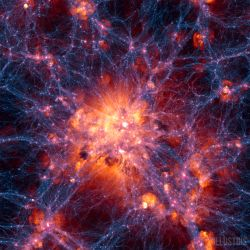
\includegraphics[trim = 0mm 3.5cm 0mm 3.0cm, clip, keepaspectratio=true,
width=0.7\textheight]{Presentation1.png}
\tiny{A projection of the cosmic web in the ILLUSTRIS simulation, that was made
with AREPO (http://www.illustris-project.org/)}
\end{center}
\tableofcontents
 
\newpage 

%============================================================================== 
\section{General Information}
\small
\subsection*{Information of the Applicant}
\begin{tabular}{L!{\VRule}R}
\bf Name		& Sebastian Bustamante Jaramillo\\
\bf Degree		& B.Sc. in Physics, Universidad de Antioquia\\
\bf Position	& PhD student. Heidelberg Institute for Theoretical Studies, Heidelberg University\\
\bf Birthday	& { 20$^{th}$ June, 1990}\\
\bf Nationality & Colombian\\
\bf Address	& Peterstaler Str. 96, 69118 Heidelberg\\
\bf E-mail 1	& macsebas33 \textit{at} gmail.com (personal)\\
\bf E-mail 2	& sebastian.bustamante \textit{at} h-its.org (academic)\\
\end{tabular}

\vspace{10pt}

More detailed information of the applicant can be found here \url{http://goo.gl/BPZGzK}

\vspace{15pt}  

\subsection*{Information of the Project}
\begin{tabular}{L!{\VRule}R}
\bf Title		& \bf Modeling supermassive Black Holes in hydrodynamical simulations of
				galaxy formation\\
\bf Field		& Cosmology, Astrophysics, Physical Sciences \\
\bf Advisor	& Professor Volker Springel. Heidelberg Institute for Theoretical Studies (HITS) 
\& University of Heidelberg, Germany \\
\bf University	& University of Heidelberg, IMPRS PhD program \\
\bf Time Frame	& 3 years \\
\end{tabular}
\normalsize
%==============================================================================


%==============================================================================
\section{Abstract}
%==============================================================================


The modelling of supermassive black holes in the center of galaxies is an important 
enterprise to be carried out as they play a central role in the current understanding
of start formation theories. However, simulating such processes in a cosmological 
context is not an easy task due to the limited numerical resolution achieved by 
current state-of-art computing systems. One of our objective is to show that at 
typically employed numerical resolutions, the orbits of sink particles used to 
represent supermassive black holes in simulations can be quite unreliable, as a 
result of two-body effects, fluctuating gravitational potentials and noisy 
dynamical friction forces. We want to test several proposals from the literature 
to improve this treatment, and suggest a new one as well. We shall use the 
improved methods to investigate how black hole recoil kicks affect the growth of 
the black hole population when black holes return to the centers of halo potentials 
on realistic timescales.


\newpage

%==============================================================================
\section{Motivation}
%==============================================================================

\subsection{First phase}

Supermassive black holes are ubiquitously observed in the centers of galaxies, 
and they play a critical role in current theories for galaxy formation, where 
they are supposed to suppress star formation in large galaxies by injecting 
energy into the gas. We hence want to simulate the growth of these black holes 
and the associated co-evolution with the galaxy when studying numerical models 
of galaxy formation. In reality, it is believed that the black holes experience 
dynamical friction against the background of dark matter and stars, and possibly 
also through gas-dynamical processes, making them spiral in to the centers of 
galaxies on a reasonably short timescale. Only when they are positioned there, 
they can efficiently influence the whole galaxy and grow rapidly. 

\

After galaxy mergers, the remnant (merged) black hole will return to the center 
through these friction processes, after being kicked out through asymmetric 
emission of gravitational waves. To properly estimate how long the growth/feedback 
may be weak/interrupted after a merger (because the center is not yet found again), 
and how many free floating massive black holes there may be, the orbit of the 
black holes needs to be followed reasonably accurately.

\subsection{Second phase}

Whenever supermassive black holes merge during galaxy mergers, they emit
a burst of gravitational wave radiation. This happens in an symmetric way such that there
is a quite large recoil, kicking the BH out of the centre. It could even happen that the BH
leaves the remnant halo entirely, but usually, it probably returns after some time. During
this period, the galaxy may then grow unimpeded by the BH. We would like to find out
how strongly predictions by galaxy formation are modified when the BH recoil kicks are
accounted for. To this end, one can apply fitting functions produced by numerical relativity
simulations to kick BH merger remnants depending on their mass ratio, whenever this
happens in a cosmological simulation (see for example Sijacki et al., MNRAS, 2011, 414,
3656, arxiv:1008.3313). Combined with a treatment of BH friction, the BHs are then
expected to return to the centers after a finite time, so that these effects can be studied in
modern simulations of galaxy formation.


%==============================================================================
\section{Problem}
%==============================================================================


Following the orbit of supermassive black holes in cosmological simulations is 
not readily possible, as the masses of dark matter and star particles in N-body 
simulation are very much larger than in reality and similar to the mass of the 
black hole. As a result, two-body scattering effects will try to 'heat-up' the 
central black hole particle and prevent it from experiencing proper dynamical 
friction, or in other words, the black hole will not return to the center of the 
potential by itself under these conditions. Current simulation models therefore 
usually employ non-physical tricks to 'glue' the black hole particle to the 
potential minimum, for example by searching for the smallest black hole potential 
value among neighbors around the black hole, and then simply positioning the black 
hole particle to this minimum. This is for example done by the Illustris and 
Gigagalaxy projects. While this prevents that the central black hole particle is 
lost, it also prevents that the above questions can be studied, and potentially 
one also introduces severe inaccuracies in the efficiency with which black holes 
can grow.


%==============================================================================
\section{Objectives}
%==============================================================================

The objectives of the project are:

\begin{itemize}

\item[\checkmark] Improving and proposing semi-analytical methods to follow 
accurately the orbit of supermassive black holes in cosmological simulations,
where dynamical friction is accounted for.

\item[\checkmark] Studying the effect of dynamical friction on the properties
of merging galaxies, e.g. how the growth and feedback of the black hole is 
strengthened, weakened or even interrupted during merging processes.

\item[\checkmark] Making statistical predictions, in a cosmological context, 
of gravitational wave emissions produced by coalescing black hole pairs.
This is very much important for current and future experiments such as LISA.
\footnote{Laser Interferometer Space Antenna for observing gravitational waves
\url{https://www.elisascience.org/}.}


\end{itemize}


%==============================================================================
\section{Methodology}
%==============================================================================


One approach for improving the modelling would be to augment the equation of 
motion for the black hole particle by an explicit dynamical friction force. 
This can be done in different ways.

\begin{itemize} 
\item One can try to add a suitably modified version of Chandrasekhar’s dynamical friction
formula, similar to how this is attempted in Tremmel et al. (2015, MNRAS, 451, 1868,
arxiv:1501.07609). This involves some assumptions and technical approximations. In the
formulation of Tremmel, they arranged it such that the force becomes ever weaker in the
limit of infinite resolution, so that one argue it is a correction for the finite resolution of real-
work simulations. However, the tests presented in the paper are not fully convincing and it
is still unclear (certainly to me), whether this method works sufficiently well in practice
(e.g. for galaxy merger simulations, and for cosmological simulations of galaxy formation).
(2) Because it not really clear whether Chandrasekhar’s formula applies well when the BH
is already close to the centre of the galaxy (where stars need to be ejected from the “loss-
cone” and interactions with gas play a very important role), one may instead also
conjecture different models. For example, if we assume that the BH is brought back
efficiently to the potential minimum if it is displaced from the centre, we can construct an
“optimum” friction force as follows: At the centre, the gradient of the potential is zero by
definition, so that it can be approximated as quadratic to first order. The BH is hence
expected to carry out harmonic oscillations around the centre. We can now try to define
an optimum damping force that eliminates the oscillation on the shortest possible
timescale (if the friction is too large, the motion will be “overdamped”, and one takes
longer to the centre than for a suitably smaller force). We can estimate the potential
around the centre as g(x) ~ phi_0 + 1/2 * (d^2phi/dx^2) * x^2, and the second derivative
along one direction can be estimated from Poisson’s equation as (d^2phi/dx^2) ~ (1/3) (4
Pi G rho), where rho is the local total mass density. The harmonic oscillator’s equation of
motion will be x’’ = - om^2 * x = - dg/dx * x, meaning that the oscillation frequency is om
= sqrt[(1/3) (4 Pi G rho)]. For a critical damping we would then need to add a friction force
as x’’ = -om^2* x - k * x’, where k = 2 * om. In this case, we expect the orbit to decay on
the local free fall timescale.
Work steps:


\end{itemize}


%==============================================================================
\section{Methodology}
%==============================================================================


The proposed project is subject to a PhD study and will cover the following 
aspects:


\begin{itemize}

\item[\checkmark] \textit{First, an analysis and characterization of existing 
hydrodynamical simulations based on the \texttt{AREPO} code will be done.}

\end{itemize}


As this project will be entirely based on numerical results, an analysis and 
characterization of existing \texttt{AREPO} hydrodynamical simulations is one 
of the key steps. This includes a quantification of the dark matter and the 
gaseous cosmic web through two different web finding schemes (i.e. the T-web 
based on the tidal tensor \citep{Hahn07,Forero09}, and the V-web based on the 
velocity shear tensor \citep{Hoffman12}, schemes in which prof. Jaime 
Forero-Romero has a broad research experience); thus voids, walls, filaments 
and clusters will be identified. Then, a statistical analysis of the found 
structures will be carried out, i.e. volume and mass filling fractions at 
different redshifts, morphology, halo populations and filamentary accretion of 
gas.


In Heidelberg, the required computer facilities and access to existing 
simulations and the private \texttt{AREPO} code (of which Prof. Volker 
Springel is the main author) is granted. Moreover, the extensive research 
expertise of Prof. Springel in numerical cosmology is 
certainly another interest for pursuing this specific PhD project.


\begin{itemize}

\item[\checkmark] \textit{Second, detailed simulations of specific processes at
high redshifts will be computed.}

\end{itemize}


Once the gaseous cosmic web is analysed, we proceed by computing its impact on 
galaxy evolution, especially at high-redshifts due to the large amount of 
available observational constraints. This step involves computing new high 
resolution \texttt{AREPO} simulations in order to study specific processes 
like: star formation rate enhanced by filamentary gas accretion, angular 
momentum exchange between galaxies and the cosmic web, spin orientation of 
galaxies along filaments and walls.


\begin{itemize}

\item[\checkmark] \textit{Third, new observables will be derived based on the
results of the simulations. }

\end{itemize}


At this point, we will compare our theoretical results with available 
observational data of the cosmic web, specifically at high redshifts. This step 
will also involve deriving new observables based on our predictions.


%==============================================================================
\section{Current State}
%==============================================================================


At present the applicant has already the fundamental knowledge in Astrophysics and
Cosmology required for this investigation. This can be confirmed by his research
experience, including a paper (as co-author) published in the \textit{ApJL} in 
which the kinematics of the Local Group in a cosmological context was studied, 
another paper (as co-author) published in the \textit{ApJ} where the influence of 
thermal evolution on the magnetic habitability of rocky planets was studied,
and some participations in academic congresses. Furthermore, a Bachelor's thesis
\footnote{\scriptsize Further information and an electronic version of this 
thesis can be found here \url{https://github.com/sbustamante/Thesis}.} where the 
preferred place of simulated Local Group-like systems in the cosmic 
web was studied, also demonstrates the ability of the applicant for handling 
simulations and massive data, a skill that is necessary for carrying out this project.

\

Currently, the applicant is also involved in two research projects: first, a 
new method for finding voids in simulations based on the local fractional 
anisotropy is investigated. An ongoing publication (as first author) related to this is about 
to be submitted\footnote{\scriptsize Information of this paper can be found 
here \url{https://github.com/sbustamante/CosmicVoidsPaper}.}. The second project
involves a comparison of three simulation techniques, i.e. \texttt{SPH} vs 
\texttt{VPH} vs \texttt{AREPO}, with possible publishable results at the end of
the present year \footnote{\scriptsize Further information in  
\url{https://github.com/sbustamante/MethodsComparison}.}.


%==============================================================================
\section{Schedule}
%==============================================================================

\begin{table}[h]
\begin{flushleft}
\begin{center}
  \begin{tabular}{l  l} \hline\hline
	\centering\textbf{Year} & \textbf{Goals} \\ \hline
	%First year
	First  
	& \tabitem Identifying a set of existing \texttt{AREPO} simulations suitable 
	for our studies. \\
	& \tabitem Applying web finding schemes (T-web and V-web) to the simulations 
	for\\
	& \ \ \ \ quantifying structures in the gaseous cosmic web, i.e. voids, walls, 
	filaments\\
	& \ \ \ \ and clusters.\\
	& \tabitem Evaluating properties of found structures at different redshifts.\\
	\\
	%Second year	
	Second
	& \tabitem Studying by means of high resolution simulations the impact of the 
	gaseous\\
	& \ \ \ \ cosmic web on specific galaxy evolution processes.\\
	\\	
	%Third year	
	Third
	& \tabitem Comparing with available observational data of the cosmic web.\\
	& \tabitem Deriving new observable from our theoretical studies.\\ 
	
	\hline\hline
  \end{tabular}  
\end{center}
\end{flushleft}
\end{table}

\newpage
%==============================================================================
\bibliographystyle{latex/mn2e}
\renewcommand{\bibname}{8\ \ \ \ Bibliography}
\small
\bibliography{references.bib}
%==============================================================================



\end{document}
